\documentclass[12pt]{article}

\pagestyle{empty}
\setlength{\topmargin}{0in}
\setlength{\headheight}{0in}
\setlength{\topsep}{0in}
\setlength{\textheight}{9in}
\setlength{\oddsidemargin}{0in}
\setlength{\evensidemargin}{0in}
\setlength{\textwidth}{6.5in}

\usepackage{palatino,graphics,amsmath,amssymb,enumitem}

\newcommand{\ds}{\displaystyle}
\newcommand{\vs}[1]{\vspace{#1in}}
\renewcommand{\vss}[1]{\vspace*{#1in}}
\newcommand{\bvec}{{\mathbf b}}
\newcommand{\cvec}{{\mathbf c}}
\newcommand{\dvec}{{\mathbf d}}
\newcommand{\evec}{{\mathbf e}}
\newcommand{\fvec}{{\mathbf f}}
\newcommand{\qvec}{{\mathbf q}}
\newcommand{\uvec}{{\mathbf u}}
\newcommand{\vvec}{{\mathbf v}}
\newcommand{\wvec}{{\mathbf w}}
\newcommand{\xvec}{{\mathbf x}}
\newcommand{\yvec}{{\mathbf y}}
\newcommand{\zvec}{{\mathbf y}}
\newcommand{\zerovec}{{\mathbf 0}}
\newcommand{\real}{{\mathbb R}}
\newcommand{\twovec}[2]{\left[\begin{array}{r}#1 \\ #2
    \end{array}\right]}
\newcommand{\ctwovec}[2]{\left[\begin{array}{c}#1 \\ #2
   \end{array}\right]}
\newcommand{\threevec}[3]{\left[\begin{array}{r}#1 \\ #2 \\ #3
  \end{array}\right]}
\newcommand{\cthreevec}[3]{\left[\begin{array}{c}#1 \\ #2 \\ #3
    \end{array}\right]}
\newcommand{\fourvec}[4]{\left[\begin{array}{r}#1 \\ #2 \\ #3 \\ #4
    \end{array}\right]}
\newcommand{\cfourvec}[4]{\left[\begin{array}{c}#1 \\ #2 \\ #3 \\ #4
    \end{array}\right]}
\newcommand{\mattwo}[4]{\left[\begin{array}{rr}#1 & #2 \\ #3 & #4 \\ \end{array}\right]}
\renewcommand{\span}[1]{\text{Span}\{#1\}}
\newcommand{\bcal}{{\cal B}}
\newcommand{\ccal}{{\cal C}}
\newcommand{\scal}{{\cal S}}
\newcommand{\wcal}{{\cal W}}
\newcommand{\ecal}{{\cal E}}
\newcommand{\coords}[2]{\left\{#1\right\}_{#2}}
\newcommand{\gray}[1]{\color{gray}{#1}}
\newcommand{\lgray}[1]{\color{lightgray}{#1}}
\newcommand{\rank}{\text{rank}}
\newcommand{\col}{\text{Col}}
\newcommand{\nul}{\text{Nul}}

\begin{document}

\noindent
{\bf Mathematics 227} \\ 
{\bf Bases}

\bigskip
A set of vectors in $\real^n$ that spans $\real^n$ and is linearly
independent is called a {\em basis} of $\real^n$.

\begin{enumerate}
\item Explain why the vectors $\vvec_1=\twovec21$ and
  $\vvec_2=\twovec12$ form a basis for $\real^2$.

  \vs{1}
  Explain why the vectors $\evec_1$, $\evec_2$, and $\evec_3$ form a
  basis for $\real^3$.

  \vs{1}
  How many vectors will be in a basis for $\real^{12}$?  Explain your
  thinking.

  \vs{1}
  Suppose that $\vvec_1,\vvec_2,\ldots,\vvec_n$ is a basis for
  $\real^n$.  Explain why every vector $\bvec$ in $\real^n$ can be
  written as a linear combination of $\vvec_1,\vvec_2,\ldots,\vvec_n$
  in exactly one way.

  \vs{1}
\item Suppose that $\vvec_1=\twovec21$ and
  $\vvec_2=\twovec12$.  The basis of $\real^2$ formed by $\vvec_1$ and
  $\vvec_2$ will be denoted by $\bcal=\{\vvec_1,\vvec_2\}$.  We now know
  that every vector in $\real^2$ can be expressed in two different
  ways:  in its usual form as a column vector and as a linear
  combination of $\vvec_1$ and $\vvec_2$.  We are going to use this to
  define a new coordinate system for $\real^2$.

  \begin{center}
    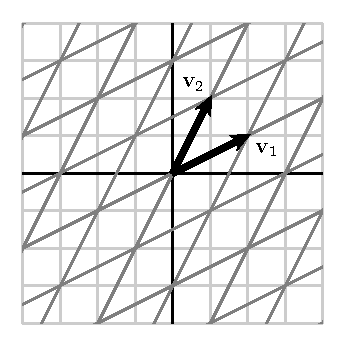
\includegraphics{basis-1.eps}
  \end{center}

  Express the vector $\twovec03$ as linear combination of $\vvec_1$
  and $\vvec_2$.

  \vs{1}
  Express the vector $2\vvec_1 - \vvec_2$ in standard form.

  \vs{1}
  If we have a vector $\xvec$ in $\real^2$, we can write
  $\xvec=c_1\vvec_1 + c_2\vvec_2$.  We will use $c_1$ and $c_2$ as new
  coordinates for $\xvec$.  For instance,
  $
  \twovec{-3}0 = -2\vvec_1 + \vvec_2$.  In the coordinate system
  defined by $\vvec_1$ and $\vvec_2$, this vector has coordinates $-2$
  and $1$.  We will write this as
  $$
  \coords{\twovec{-3}0}{\bcal} = \twovec{-2}1.
  $$
  In general, if $\xvec=c_1\vvec_1+c_2\vvec_2$, then
  $$
  \coords{\xvec}{\bcal} = \twovec{c_1}{c_2}.
  $$

  Express $\twovec{-4}1$ as a linear combination of $\vvec_1$ and
  $\vvec_2$ to find the coordinates $\coords{\twovec{-4}1}{\bcal}$.

  \vs{1}
  \newpage
  Find the vector $\xvec$ so that $\coords{\xvec}{\bcal} =
  \twovec2{-3}$.

  \vs{1}
\item Explain why the vectors
  $$
  \vvec_1=\threevec10{-2},\hspace*{24pt}
  \vvec_2=\threevec{-2}1{0},\hspace*{24pt}
  \vvec_3=\threevec112
  $$
  form a basis $\bcal$ for $\real^3$.

  \vs{1}
  Find the vector $\xvec$ such that $\coords{\xvec}{\bcal} =
  \threevec2{-1}{-2}$.

  \vs{1}
  Find the coordinates $\coords{\threevec{-2}{1}{-8}}{\bcal}$.

  \vs{1}
\item Suppose that $\bcal$ is the basis for $\real^2$ consisting of
  the vectors $\vvec_1=\twovec21$ and
  $\vvec_2=\twovec12$.  Let's form the matrix
  $$A=\left[\begin{array}{cc}\vvec_1 & \vvec_2 \\ \end{array}\right]
  =\mattwo2112.$$

  \newpage

  Explain why $A\coords{\xvec}{\bcal} = \xvec$.

  \vs{1.5}
  Find a matrix $B$ such that $B\xvec = \coords{\xvec}{\bcal}$.
  
  
    

  
              
    
    


\end{enumerate}


\end{document}
